\newpage

\textbf{Komponenten\hyperlink{}{/LFxx/}} \\

\paragraph{PCM5102a Breakout Board}

\begin{wrapfigure}{r}{0.4\textwidth} % Increase the width of the figure environment
	\vspace{-20pt}
	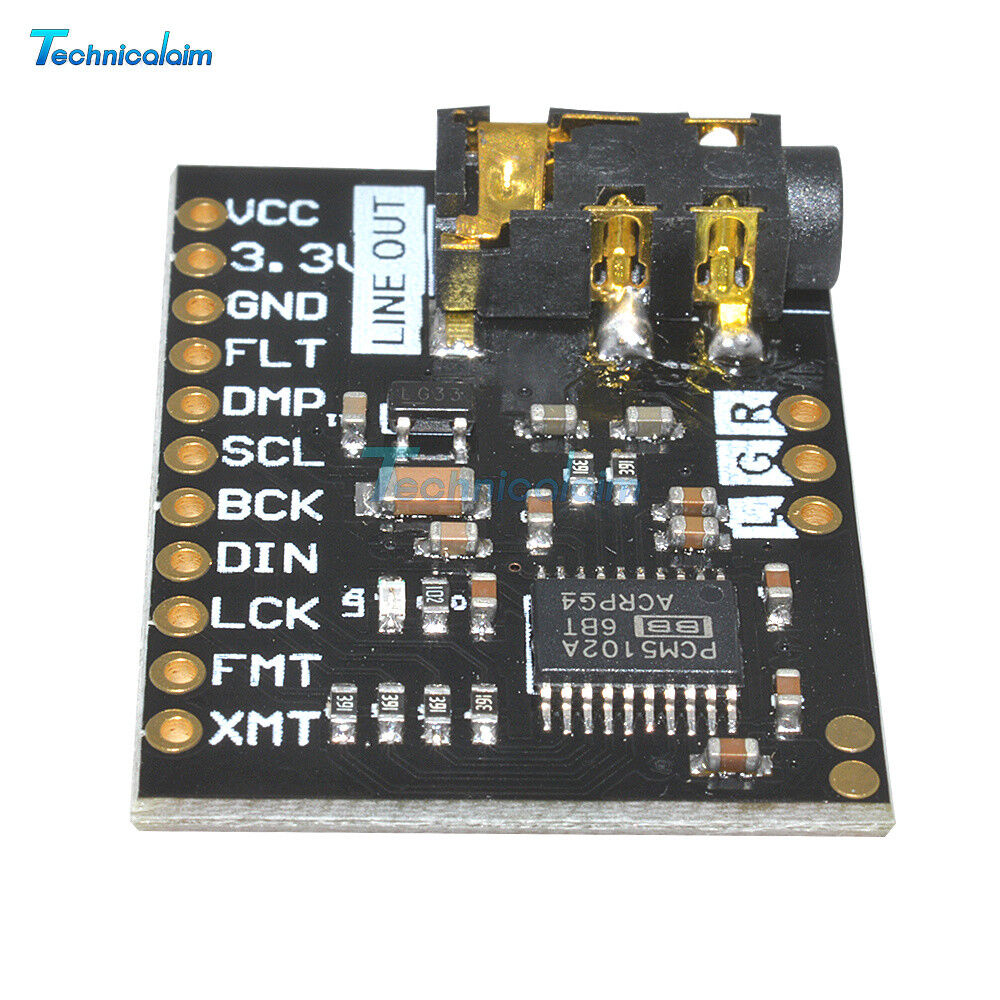
\includegraphics[width=0.2\textwidth]{images/05_technische_spezifikation/audio/pcm5102a_breakout.jpg}
	\caption{PCM5102a Breakout Board}
	\label{fig:pcm5102a_breakout}
\end{wrapfigure}

Der PCM5102a Audio Codec wurde für die DAC Wandlung der Audiodaten verwendet. Für die Implementation und die Entwicklung des Prototyps wurde ein Breakout Board gekauft, um ohne die Notwendikeit eines PCB-Design die Firmware für \textbf{I M A} zu schreiben. 
Komfortablerweise ist direkt eine \SI{3,5}{\milli\meter} Stereo-Klinkenbuchse auf dem Board verbaut.
Der Pegel beträgt Line-Level (\SI{\pm 1.7}{\volt_{rms}}), und ist somit grob kompatibel zum Eurorack-Standard.

Das PCB-Design inklusive aller Komponenten sollte dann auf die Entwicklung der Firmware folgen, wurde aber aus dem Featureumfang des Projektes wegen Zeitknappheit gestrichen.

Anfänge des PCB-Designs wurden bereits in KiCad entwickelt.
Die Levelshifting Schaltungen für die Umwandlung von Eurorack Leveln \SI{\pm 5}{\volt} zu den Pegeln des Audio Codecs \SI{\pm 0.7}{\volt_{rms}} wurden bereits entwickelt (siehe Anhang \ref{sec:appendix}).

Das Breakout Board wird mit einer Versorgungsspannung von \SI{3,3}{\volt} betrieben.

Als Übertragungsprotokoll dient \textbf{I2S}. Die detaillierte Inbetriebnahme findet sich in Abschnitt \ref{sec:pcm5102a-und-i2s}.


\paragraph{Waveshare Micro SD-Card Module}

\begin{wrapfigure}{r}{0.4\textwidth} % Increase the width of the figure environment
	\vspace{-20pt}
	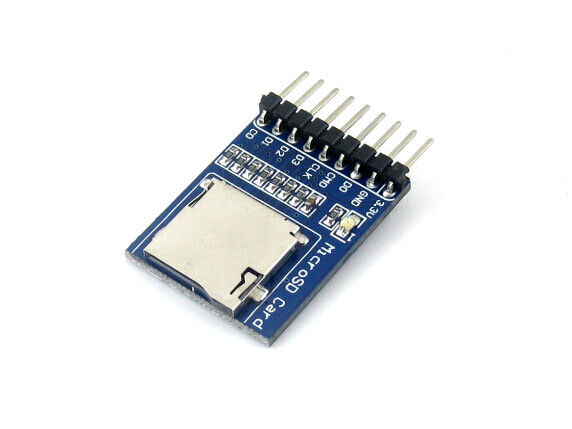
\includegraphics[width=0.4\textwidth]{images/05_technische_spezifikation/audio/waveshare_micro_sd_module.jpg}
	\caption{Waveshare Micro SD-Karten Modul}
	\label{fig:waveshare_micro_sd_module}
\end{wrapfigure}

Das Waveshare Micro SD-Card Module wird für die Speicherung und den Zugriff auf Audiodaten in diesem Projekt verwendet. Dieses Modul ermöglicht die einfache Integration von Micro SD-Karten in das System, um persistente Daten zu lesen und zu schreiben, ohne aufwändige PCB-Designs oder zusätzliche Hardwarekomponenten implementieren zu müssen.

Das Modul unterstützt den Standard \textbf{SDIO}-Bus zur Datenübertragung, was eine einfache Anbindung an das Mikrocontroller-System ermöglicht. 

Die Inbetriebnahme und die spezifischen Konfigurationen für die Verwendung dieses Moduls werden in Abschnitt \ref{sec:sd-card-audio} detailliert beschrieben. 

Das Modul wird mit einer Versorgungsspannung von \SI{3.3}{\volt} betrieben.

\newpage
\subsubsection{Pinout Audio Komponente}

\textbf{Audio}
\begin{longtable}[c]{|p{2.5cm}|p{1cm}|p{2.5cm}|p{2.5cm}|p{2.5cm}|p{3cm}|}
	\hline
	\textbf{Komponente} & \textbf{PIN} & \textbf{Signal-On-PIN} &  \textbf{GPIO-Mode} & \textbf{GPIO-Pull-Up/Pull-Down } & \textbf{User-Label}\\
	\hline
	SDIO & PC8 & SDIO\_D0 & AFPP & PULL UP & n/a \\
	\hline
	& PC9 & SDIO\_D1 & AFPP & PULL UP & n/a \\
	\hline
	& PC10 & SDIO\_D2 & AFPP & PULL UP & n/a \\
	\hline
	& PC11 & SDIO\_D3 & AFPP & PULL UP & n/a \\
	\hline
	& PC12 & SDIO\_CK & AFPP & NPU NPD & n/a \\
	\hline
	& PD2 & SDIO\_CMD & AFPP & PULL UP & n/a \\
	\hline
	I2S & PB10 & IS2\_CK & AFPP  & NPU NPD & n/a \\
	\hline
	& PB12 & IS2\_WS & AFPP & NPU NPD & n/a \\
	\hline
	& PC3 & IS2\_SD & AFPP & NPU NPD &  n/a \\
	\hline
	& PC6 & IS2\_MCK & AFPP & NPU NPD &  n/a \\
	\hline
\end{longtable}

\textbf{NPU NPD} = No Pull Up No Pull Down		

\textbf{AFPP} = Alternate Function Push Pull 

